
Aurélie fait du vélo en Angleterre au col de Hardknott.

Elle est partie d'une altitude de 251 mètres et arrivera au sommet à une altitude de 393 mètres.

Sur le schéma ci-dessous, qui n'est pas en vraie grandeur, le point de départ est représenté par le point A et le sommet par le point E. Aurélie est actuellement au point D. 

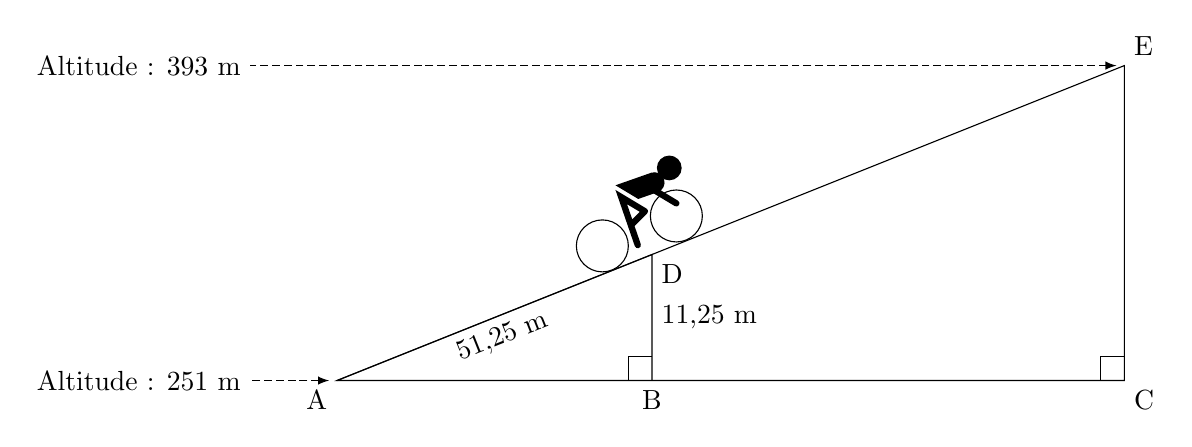
\begin{tikzpicture}
	\draw (0,0) node [below left] {A} -- (10,0) node[below right] {C} -- (10,4) node[above right]{E} -- cycle;
	
	\draw[dash pattern = on 1mm off 0.5mm, <-,> = latex] (-0.1,0)-- (-1.1,0) node [left]{Altitude : 251 m};
	
	\draw[dash pattern = on 1mm off 0.5mm, <-,> = latex] (9.9,4)-- (-1.1,4) node [left]{Altitude : 393 m};
	
	\draw (0,0) -- (4,1.6) node[pos=0.5, sloped, below] {51,25 m} node [below right]{D} -- (4,0) node[pos = 0.5, right]{11,25 m} node[below] {B};
	
	\draw (3.7,0)--(3.7,0.3)--(4,0.3) (9.7,0)--(9.7,0.3)--(10,0.3);
		
%	\draw[shift={(4,1.6)}, line width = 0.8 mm, line cap = round, line join = angle] (-0.09,0.06) -- (-0.2,0.37)--(0.05,0.28)--(-0.12,0.2);

\draw [shift={(4,1.6)},line width=3.2pt,fill=black,fill opacity=1.0] (0.22,1.1) circle (0.1);
\draw [shift={(4,1.6)}]  (-0.63,0.11) circle (0.33) (0.31,0.49) circle (0.33);

	\draw [shift={(4,1.6)}, line width = 0.8 mm, line cap = round, line join = angle] (-0.18,0.12)--(-0.39,0.73) -- (-0.09,0.55) (-0.09,0.55) -- (-0.25,0.39);

	\draw [fill=black, shift={(4,1.6)}, line width = 0.8 mm, line cap = round, line join = angle] (-0.37,0.87) -- (0,1) arc (109:-71:0.09) -- (-0.17,.75)-- cycle;
	
	\draw [fill=black, shift={(4.4,1.7)}, line width = 0.8 mm, line cap = round, line join = angle]	(-0.39,0.73) -- (-0.09,0.55);
	
	%(0.21,0.62) -- (-0.28,0.82) ;
\end{tikzpicture}

Les droites (AB) et (DB) sont perpendiculaires. Les droites (AC) et (CE) sont perpendiculaires. Les points A, D et E sont alignés. Les points A, B et C sont alignés.

AD = 51,25 m et DB = 11,25 m.

\begin{enumerate}
	\item Justifier que le dénivelé qu'Aurélie aura effectué, c'est-à-dire la hauteur EC, est égal à $142$~m.
	
	\item \begin{enumerate}
		\item Prouver que les droites (DB) et (EC) sont parallèles.
		\item Montrer que la distance qu'Aurélie doit encore parcourir, c'est-à-dire la longueur DE, est d'environ 596 m.
	\end{enumerate}
\item On utilisera pour la longueur DE la valeur 596 m.
	
Sachant qu'Aurélie roule à une vitesse moyenne de 8 km/h, si elle part à 9~h~55 du point D, à quelle heure arrivera-t-elle au point E ? Arrondir à la minute.
	
\item La pente d'une route est obtenue par le calcul suivant :
	
	\begin{tabularx}{\linewidth}[t]{@{}X@{\qquad}| l|} \cline{2-2}
	
$\text{pente} =	\dfrac{\text{dénivelé}}{\text{longueur horizontale parcourue}}$.
	
La pente s'exprime en pourcentage.
	
Démontrer que la pente de la route parcourue par Aurélie est de 22,5\,\%.&
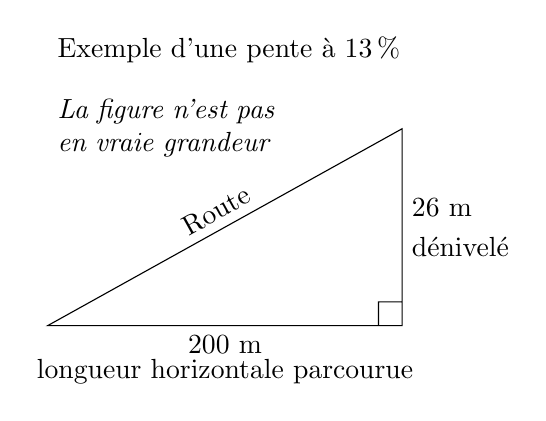
\begin{tikzpicture}[baseline={(t)}]
	 \node (t) at (0,3.5) [right] {Exemple d'une pente à 13\,\%};
	 \node (d) at (0,3) [below right, text width = 3 cm] {\emph{La figure n'est pas en vraie grandeur}};
	 \draw (0,0)--(4.5,0) node [pos = 0.5, below] {200 m} node [pos = 0.5, below=3mm] {longueur horizontale parcourue}--(4.5,2.5) node [pos = 0.4, right]{dénivelé} node [pos = 0.6,right]{26 m}--cycle node[sloped, pos = 0.5, above] {Route}
	 (4.2,0) -- (4.2,0.3)--(4.5,0.3);
\end{tikzpicture} \\ \cline{2-2}
\end{tabularx}
\end{enumerate}

\vspace{0,5cm}

